\documentclass{article} % For LaTeX2e
\usepackage{nips11submit_e,times}
\usepackage[lined,boxed,commentsnumbered]{algorithm2e}
\usepackage{amsmath}
\usepackage{graphicx}
\usepackage{url}
\usepackage{multirow}
%\documentstyle[nips10submit_09,times,art10]{article} % For LaTeX 2.09


\title{Predicting the Tags of Questions in StackOverflow}

\newcommand{\fix}{\marginpar{FIX}}
\newcommand{\new}{\marginpar{NEW}}

%\nipsfinalcopy % Uncomment for camera-ready version

\begin{document}

\maketitle

\begin{abstract}
In a tagging system, users can add metadata in the form of keywords to shared content. In these years, tagging system has been widely used in many websites that highlights user-generated content. In this project, we focus on the tags prediction of a untagged document.Specifically, we apply our prediction methods to StackOverflow.com, the world's largest programmer Q\&A community.

In this project, we address these problem by Naive Bayes model and k Nearest Neighbors model. Especially, with the analysis of the strength and weakness of the original approaches, we proposed improvements on both models, which significantly promoted the overall performance of the tag prediction. As the experimental results indicates, the proposed models outperformed the baseline method by over 20\% in both recall and precision.

\end{abstract}


As the world's most popular programmer Q\&A community, StackOverflow.com is a showcase of the successful usage of the tagging system, where each question could have one or more tags to indicate its ``topics". 

Traditional hierarchical taxonomies force each item to be one of the predefined categories, however in a tagging system one item could have multiple categories(the ``tags"). Moreover, the tagging systems normally encourages users to contribute their own tags. Thus, by gathering the ``wisdom of the crowd", an item can have more up-to-date and precise descriptors.

In this project we aim at predicting the tags of a question by analyzing the tagged questions/answers from StackOverflow.com. That is, given a question, our system will predict appropriate tags for it. With the tag predictor, a user could have suggested tags at hand as soon as he/she asked a question. This will facilitate tagging task. Sen et al.\cite{Sen2006} point out that with suggestion people are more likely to assign items with higher quality tags.

Moreover, the tag prediction will also benefit the already tagged questions by giving us a deeper insight into that question in the following ways:

\begin{itemize}
    \item Reveal the hidden tags: often a piece of text is a mix of different topics while a user may only choose a fraction of them as the tags. That is to say, these tags only indicate the ``partial topics" of the text. With the tag prediction technology, we're able to discover the ``hidden" tags.
    \item Discover the Vocabulary difference: different users may use different terms to describe the same item. Our predictor can be a good assistant in finding the synonym tags because similar tag by searching tags with similar word distribution.
    \item Disambiguation: tags are short and often ambiguous. With additionally predicted tags it will easier grasp the meaning of a specific tag. For example, an article with tag ``apple" may tell us little of its content, but if we find the hidden tags ``osx", ``iphone" then we know exactly what ``apple" mean under such context.
\end{itemize}

In this project, we will adopt and improve several methods to predict the tags of the questions in StackOverflow.com. Unlike traditional classification problems, tag assignment is harder owing to its subjectivity and incompleteness. We'll discuss more about this in experiment section.



\subsection{Tagging System}
\subsection{Text Classfication}
\subsection{Social Tag Prediction}


\section{Proposed Methods}
\subsection{Simple Matching}
To begin with, we proposed a simple matching method as our baseline. It requires no previous knowledge of training samples. Given a test sample, the algorithm simply tries to match each word in the test sample with the list of tags. If the word exists in the tag list, the algorithm put this word as one of the candidate tags. Then the candidate tag list is sorted in descending order based on the frequency of tags in the train set, denoted as $F(Y)$, and output the top $k$ tags in the list. If the list is not full, then the algorithm fills the list up by picking tags in the remaining tag list with maximum $F(Y)$. The algorithm is described in Algorithm \ref{alg:sm}.

\IncMargin{1em}
\begin{algorithm}
\label{alg:sm}
\SetKwInOut{Input}{Input}\SetKwInOut{Output}{Output}
\Input{Frequency of tags $F(Y)$, constant $k$, test case $X_t$}
\Output{Sorted list of predicted tags $L$ for $X_t$}
\BlankLine
Initialize $L \leftarrow \emptyset$ \;
\ForEach{$x_i \in X_t$} {
	\If{$F(x_i) \neq 0$}{
		put $x_i$ in $L$ \;
	}
}
Sort $l_i \in L$ in descending order by $F(l_i)$ \;
\If{$size(L)>k$}{
	Remove all elements $l_i$ that $i \geq k$ \;
}
\While{$size(L)<k$}{
	Pick a tag in the remaining tags with maximum frequency \;
}
\Return $L$\;
\caption{Simple Matching Algorithm}\label{algo_disjdecomp}
\end{algorithm}
\DecMargin{1em}

\subsection{Naive Bayes}
Naive Bayes classifier is a simple yet powerful classifier based on Bayes theorem. It assumes that the presence of one feature is independent from the presence of the others. When performing the text categorization, Naive Bayes treats each document as a ``bag of words" and words are conditionally independent from each other.

In practice, naive Bayes classifiers can have a very satisfactory performance in a supervised learning. Many real-world problems are tackled by naive Bayes. Owing to its simplicity and desirable accuracy in many cases, we chose naive Bayes as our baseline. In our tagging prediction problem, we view the words as the features and tag the labels.

By applying Bayes theorem, we can get the label $Y$'s probability given $X$.
\begin{gather}
    P(Y \vert X_1,\dots,X_n) = \frac{P(Y) \ P(X_1,\dots,X_n\vert Y)}{P(X_1,\dots,X_n)}. 
\end{gather}

With the independence assumption, the classification problem is equivalent to:
\begin{gather}
    \mathrm{y} = \underset{y}{\operatorname{argmax}} \ P(Y=y) \displaystyle\prod_{i=1}^n P(X_i=x_i\vert Y=y).
\end{gather}
The training algorithm is stated in Algorithm \ref{alg:nb}.

\IncMargin{1em}
\begin{algorithm}
\label{alg:nb}
\SetKwInOut{Input}{Input}\SetKwInOut{Output}{Output}
\Input{Training set $T=\{t_1,...t_n\}$}
\Output{$P(Y)$ and  $P(X|Y)$}
\BlankLine
Initialize all $Count(y)$ and $Count(x|y)$ to be 0\;
Initialize total count $N$ to be 0\;

\ForEach{$t \in T$} {
    $X_t, y_t$ = $t$\;
    \ForEach{$x \in X_t$} {
        $Count(y) \leftarrow Count(x) + 1$ \;
        $Count(x|y) \leftarrow Count(x|y) + 1$ \;
        $N \leftarrow N$ + 1 \;
    }
}
% Calculate $P(Y), P(X|Y)$ from $Count(Y), Count(X|Y)$ and $N$}
\Return $P(Y), P(X|Y) \leftarrow CalculateProbability(Count(Y), Count(X|Y), N)$

\caption{Naive Bayes Training Algorithm}\label{algo_disjdecomp}
\end{algorithm}
\DecMargin{1em}

With the calculated $P(Y) and P(X|Y)$, we can apply the MLE(or MAP) to find the top-rank tags.

\subsection{k-Nearest Neighbor}

The $k$-nearest neighbor algorithm\footnote{http://en.wikipedia.org/wiki/K-nearest\_neighbor\_algorithm} ($k$-NN) is a method for classifying objects based on closest training examples in the feature space. It is type of instance-based learning where the function is only approximated locally and all computation is deferred until classification. The training phase of this algorithm consist only of storing the feature vectors and the classification labels. In the classification phase, a test case is assigned with the most frequent labels among the the nearest $k$ training samples. The distance between two feature vectors is measured by some specific metrics and $k$ is a user-defined constant value.

By applying this method to our problem, our intuition is that similar questions will have similar tags. We use cosine similarity to measure the closeness of two feature vectors. The definition is as follows:

\begin{gather}
	CosSim(P,Q)=\frac{\sum_{t \in V}w_P(t)w_Q(t)}{\sqrt{\sum_{t \in V}w_P(t)^2 \sum_{t \in V}w_Q(t)^2}}
\end{gather}

where $w_P(t)$ and $w_Q(t)$ are the weights of the term $t$ in feature vector $P$ and $Q$, respectively. We remove stopwords and stem the remaining tokens before computing the similarity score. And we use \textbf{lnn} term weights (i.e. logarithmic term frequency, no tag frequency, no normalization). For example, $w_P(t) = 1 + log(f_P(t))$ where $f_P(t)$ is the frequency count of term $t$ in vector $P$. The algorithm for k-NN is stated in Algorithm \ref{alg:knn}.

\IncMargin{1em}
\begin{algorithm}
\label{alg:knn}
\SetKwInOut{Input}{Input}\SetKwInOut{Output}{Output}
\Input{Training set $T=\{X_1,...X_n\}$, constant $k$, test case $X_t$}
\Output{Sorted list of predicted tags $L$ for $X_t$}
\BlankLine
Initialize $L \leftarrow \emptyset$ and $scoreList \leftarrow \emptyset$\;
\ForEach{$X_i \in T$} {
	$score \leftarrow CosSim(X_i, X_t)$ \;
	$scoreList_i \leftarrow score$ \;
}
Sort $s_i \in scoreList$ in descending order \; 
Put the tag of $s_0, s_1, ..., s_{k-1}$ in $L$ \;
\Return $L$\;
\caption{k-Nearest Neighbor Algorithm}\label{algo_disjdecomp}
\end{algorithm}
\DecMargin{1em}



\section{Experiments}

\subsection{Dataset and Evaluation Methods}
The dataset used in our experiments is provided by StackOverflow.com. Currently, there are 2.2 million questions, 4.8 millions answers, over 35 thousands tags in this dataset\cite{DataDump}.

We prepared 1,050,000 posts (a post is either a question or an answer)  as the training data $S_{train}$. Also we randomly sampled 5 groups of test data, each with 1000 posts.$S_{test}^i, i \in [1, 5]$.

In our experiments, precision and recall are the metrics to evaluation the predicted results. Here is the definition of the \emph{precision} and \emph{recall}:
$$ \text{Precision}=\frac{tp}{tp+fp}, \text{Recall}=\frac{tp}{tp+fn} $$
where $tp$ is the number of true positive samples, $fp$ is the number of false positive samples and $fn$ is the number of false negative samples.

As we mentioned in \emph{Introduction}, the big challenge of tag prediction is that tags are often quite subjective and incomplete. As a result, it will be problematic to conclude that a tag is "correctly" predicted only when it appears in user-defined tags. For example, if a question is tagged with "java" but predicted tag is "jdk", we still believe it is a \emph{"good"} prediction because in real life, "jdk" is closed related with "java".

Thus, instead of measure the "goodness" of a tag with only \emph{match/unmatch}, we assign each predicted tag with a relevance score $s, s \in [0, 1]$. The higher the score, the more
relevant two tags are.

To get the relevance score $s$, we proposed two methods:
\begin{itemize}
    \item{Kullback-Leibler divergence}: Kullback–Leibler is an asymmetric measure of the difference between two probability distributions $P$ and $Q$. In our case, each tag has a corresponding \emph{word distribution} and we assume that similar tags will often have similar word distribution.
    \item{Co-occurrence rate}: an alternative way for the similarity measurement is to calculate the co-occurrence rate between predicted tags and user-defined tags. Co-occurrence is asymmetrical and is very suitable to infer from sub-type tag to parent-type tag. For example, with co-occurrence rate, the predicted tag "jdk" is very relevant to user-defined tag "java". However, the co-occurrence rate from "java" to "jdk" will be much smaller.
\end{itemize}

These tools enable automatic test and thus ease the evaluation on large test set.

\subsection{Experimental Results}
\subsubsection{Naive Bayes}
In naive Bayes, we choose the top-rank $N$ tags as our predicted tags. Figure \ref{fig:naive} shows the precision/recall of Bayes classifier with different $N$. We can see that the recall increases as $N$ goes up; whereas the precision drops when $N$ increases.

\begin{figure}[htb!]
\centering%
    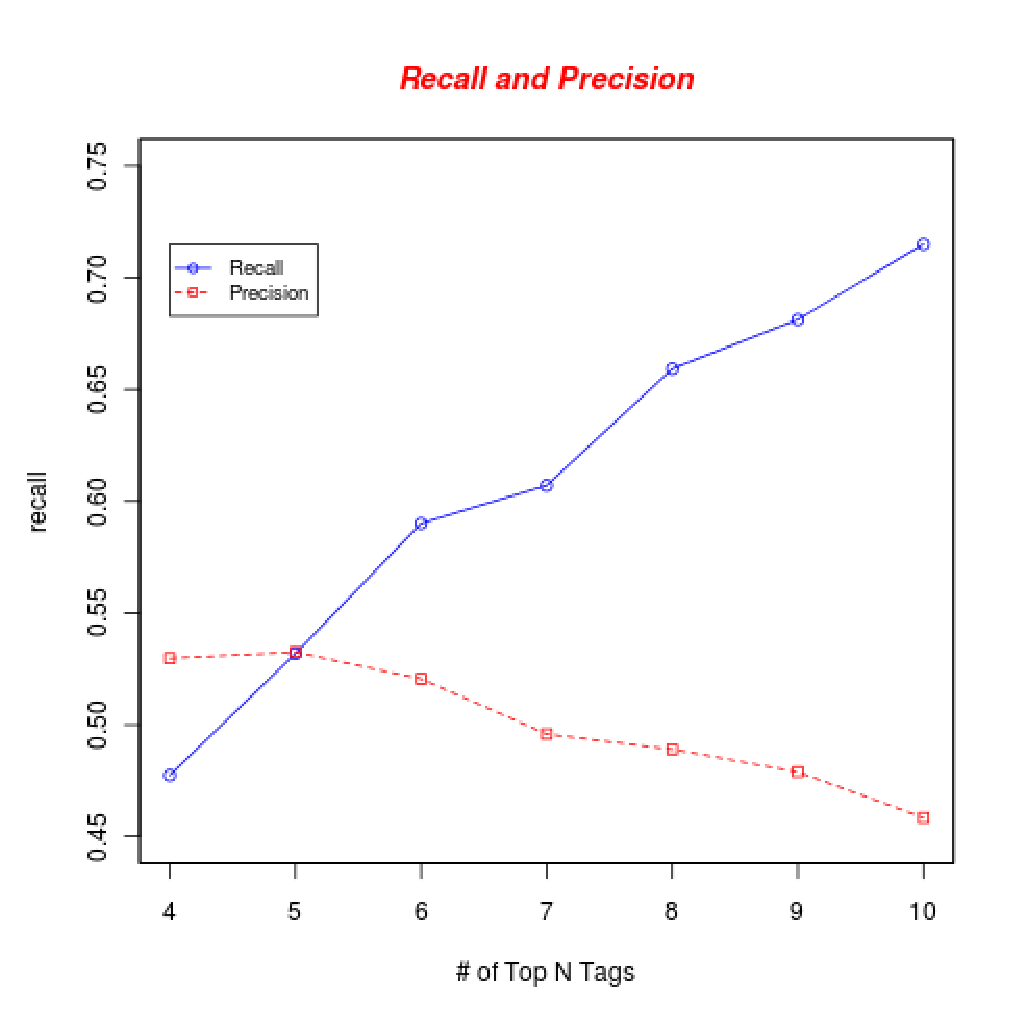
\includegraphics[scale=0.42]{naives.eps}
\caption{Tag Prediction By Naive Bayes}
\label{fig:naive}
\end{figure}

\subsubsection{Logistic Regression}
Under Construction

\subsubsection{Neural Networks}
Under Construction

\subsection{Comparison and Conclusion}
Under Construction. This part depends on the experimental results of all the three models.


\section {Future Work}
Our work has untapped an interesting area of social tagging. We believe that tag prediction is not trivial because it can be used in many applications. Here are a few possible scenarios:
\begin{itemize}
    \item \emph{Tag Suggestion:} When a user is posting a new question, the system can suggest tags for the given content.
    \item \emph{Discover the ``hidden" tags:} User-defined tag maybe subjective and incomplete. The tag predictor could be used to discover the ``hidden" tags. Moreover, with more tags being found the system can better match a question and a user's preference.
\end{itemize}



\small{
\bibliography{ref}
\bibliographystyle{plain}
}

\end{document}
